\documentclass[conference]{IEEEtran}
\IEEEoverridecommandlockouts
% The preceding line is only needed to identify funding in the first footnote. If that is unneeded, please comment it out.
\usepackage{cite}
\usepackage{amsmath,amssymb,amsfonts}
\usepackage{algorithmic}
\usepackage{graphicx}
\usepackage{textcomp}
\usepackage{xcolor}
\usepackage{array}
\def\BibTeX{{\rm B\kern-.05em{\sc i\kern-.025em b}\kern-.08em
    T\kern-.1667em\lower.7ex\hbox{E}\kern-.125emX}
    references}
\begin{document}

\title{Analysis of Dataset\\
}

\author{\IEEEauthorblockN{1\textsuperscript{st} Justo V. Andrey}
\IEEEauthorblockA{\textit{Dep. Computer Science} \\
\textit{Unifesp}\\
São José dos Campos, Brazil \\
ajusto@unifesp.br}
}

\maketitle

\begin{abstract}
This research will describe a study to classify design pattern using fine-tuning.
\end{abstract}

\begin{IEEEkeywords}
design patterns, llm, fine-tuning, neural network, transformers, Semi-supervised training
\end{IEEEkeywords}

\section{Introduction}

This study is focused in get public code from the internet and classify it based on the design pattern used.

We will be developing a protocol to train and classify the model using semi-automated\cite{5291929}(SST) approach and use fine-tuning with UniXcoder\cite{guo2022unixcoder}.
This study will be organized by describing the literature review explaining how design patterns works and the importance of those in software engineering. 
Then, we will describe how we generated our dataset used in training phase. Also we will, describe semi-automated training approach, UniXcoder transformer and fine-tuning.
After, we will describe the methodology used in our study describing how we implemented the classification and how we make experiments to evaluate it showing the results.
Finally, we will discuss the about the approach and exemplify future work.

\section{Literature Review}

\subsection{Design Patterns}

In the real world, we may found similiar problems happened. Those problems may be solved using common solutions or ideas.
Describing the process to solve such repetitive problem and representing them in code can be called as Design Patterns. 
The concept was first described in \cite{AlexanderEA.1977}, defining a structure to design an urban environment. 
This idea was introduced in software engineering by \cite{gamma1994design} applying patterns to programming.

Design Patterns are standards used in software engineering to solve common and well-know sub-problems of the real world.
Usually they focus on improving architectural characteristics like, readability, maintainence, extensibility, portability, decouple code or even testing.
Aditionally, implementing the right design pattern can enable creation of new features, provide good standards for developers to evolve code, improve cost savings and non-functional requirements \cite{988711}.

Patterns are different from algorithms, because algorithms are defined by well formed steps that a computer can execute\cite{}.
In the other hand, Design Patterns offers a high-level definition of the solution, which means the code may differ when applying the same pattern for different programs. 
They define a Design pattern using an intent to define which kind of problem we aim to solve, a motivation which emphasis a particular functional requirement or non-functional requirement, an structure or pseudocode to define how it fits on real world problems and an example of real implementation.

Generally, it's not straightforward to identify such class of problems, but once we can find their repetition in systems, then we can describe then as Design Patterns.

Even studying this class of problems for years\cite{}, it may not be simple to apply those patterns. 
This happens because in real world, we have other factors that impact implementation of systems. 
First of all, programs are different because they were made by different people, organizations are different, cultures around the teams may be different as well and resources available like, time, money or technical limitations may differ.
Such theme is really important to software engineering that even books like, \cite{}, are written about it.

Some studies like, \cite{4493325} and \cite{4301130} shown disadvantages of over-using design patterns arguing that it may increase difficulties on software evolution.

Unfortunately, there is no common consensus if design patterns are really enabling better quality or if they are making software harder to maintain. 
This happens due to the fact that it is not simple and objective to compare studies related to software quality, because usually there are many differences in design study and execution\cite{RIAZ201514}.


\subsection{Semi-supervisioned Training}

Training machine learning models is a crucial piece of development of new technologies that involves giving data to the algorithm to learn patterns or even learn possible outputs as are called labels.
Engineers do not implement all possible logic and pieces of internal software to make it useful rather than that we leverage math and statistical models to learn such things.

One of the most expensive and valuable pieces of this development is data. Data is need to make such algorithms really learn patterns that may be simple for humans to understand.
Because of that we have two main types of training. The first, the supervised training, which is when we not only give the data as input, but also we know what that data represents, this data is called labeled data.
The second one, the unsupervised training, which is when we provide the data, but we don't add any information that how it should predict and we let the algorithm learn the patterns based on input and parameters.
The first one, is simple to validate, only getting parts of the training data and using them not for training but to check if predictions are the expected ones.
The second one, could be harder to validate, since it's needed to represent the predictions somehow, usually we try to plot those in 2D graphs, heatmaps and try to understand if that data that is closed should be there.
Finally, supervisioned training is cost expensive since we need an expert to organize and label the data before training. Unsupervised is simpler because it's only needed to find the data without understanding what it means.

Both types of training have benefits and challenges, in this sense if we combine both of them in a process that we can apply supervisioned training first, we can label a small dataset and train a model. 
After that, applying unsupervisioned training, we can fetch data and use the intermediated model to predict it's label.

In that sense, to apply the supervisioned training we need to find public code and classify them manually focusing only on the design patterns on table 1.

\begin{table}[htbp]
    \caption{Design Patterns used in manual classification}
    \begin{center}
        \begin{tabular}{|c|c|}
            \hline
            \textbf\textbf{\textit{Design Pattern}}& \textbf{\textit{Label}} \\
            \hline 
            Abstract Factory & abstract\_factory \\
            \hline 
            Adapter & adapter \\
            \hline 
            Builder & builder \\
            \hline 
            Chain Of Responsibility & chain\_of\_responsibility \\
            \hline
            Decorator & decorator  \\
            \hline
            Facade & facade  \\
            \hline
            Feature Flags & feature\_flags \\
            \hline
            Observer & observer  \\
            \hline
            Singleton & singleton  \\
            \hline
            Strategy & strategy  \\
            \hline
            Unknown & unknown  \\
            \hline
        \end{tabular}
        \label{tab1}
    \end{center}
\end{table}

This process is highly time demanding, in this sense we labeled 153 to train our model, get new data and label those using predictions and iterating over this.
After this process we got more 1000 examples to increment our dataset.

This approach is been used for images as described in \cite{5291929}, but recently we have found new studies related to coding classification and querying as mentioned in \cite{9689884}. 
It allows researchers to grow the dataset without increasing too much prediction errors and because we have more data our model will have improved accuracy and f1-score.

\subsection{UniXcoder}

UniXcoder is a pre-trained model for programming languages and natural languages developed in 2022, this model was made from BERT\cite{Devlin2019BERTPO}. 
The model supports text to code, code to text, code to code. 

UniXcoder was made using same concepts as BERT \cite{Devlin2019BERTPO}, which uses a transformer architecture. 

\begin{figure}[ht]
    \centering
    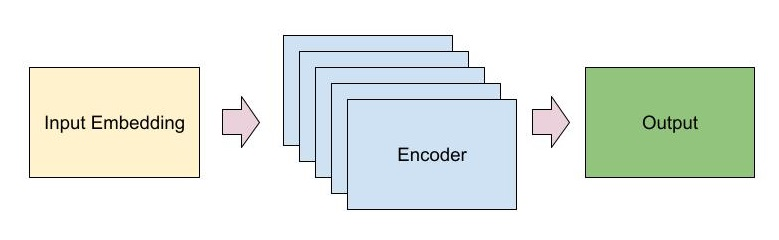
\includegraphics[scale=0.42]{./imgs/unixcoder-arc.jpg}
    \caption{UniXcoder simplified architecture}
\end{figure}

As we can see in the figure 1, one of the challenges is to represent data in a way the model can understand it.
Data has a lot of ways to be interpreted and it could generate errors or even for code syntax problems.
That's what we call input embedding or code embedding. This approach let algorithms to represent data or code as data in dense vectors of numbers in a continuous space.

\begin{figure}[ht]
    \centering
    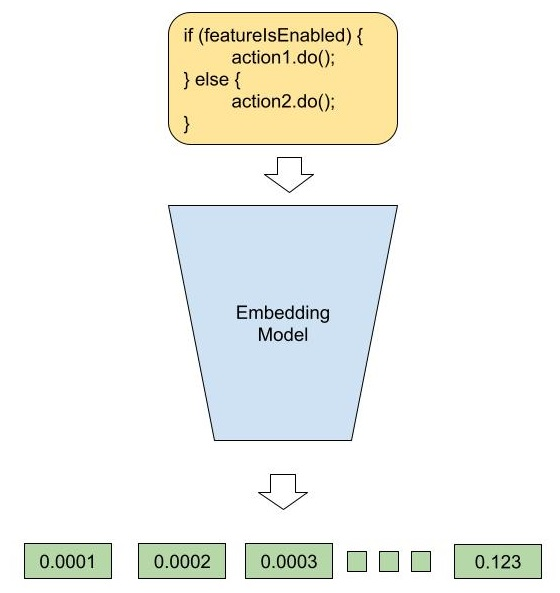
\includegraphics[width=8.5cm, height=10cm]{./imgs/code-embedding.jpg}
    \caption{Code Embedding Example}
\end{figure}


This representation can show hidden information in the code, for example semantic and functional relationships which are very important when humans need to understand code.
For example, as described in the research \cite{9463106} which uses CodeBERT\cite{feng-etal-2020-codebert} to automate program repair for Java. 

UniXcoder uses BERT as base and has 3 modes. It can be used only with encoders for code searching and similarity check, if used as decoder, it can do code generation from a input code and finally if used as encoder-decode, the model can take a code as input and summarize it or give a function name or even make API recommendations.

\subsection{Fine-tuning}

fine-tuning allows us to use pre-trained models to enrich predictions with additional data.
This process makes new subjects to be more precise, easier and faster to train. 

First we need to find a pre-trained model that suits our needs, then with labeled data we can retrain this model generating a custom model, figure 3 exemplify the idea of this process.

\begin{figure}[ht]
    \centering
    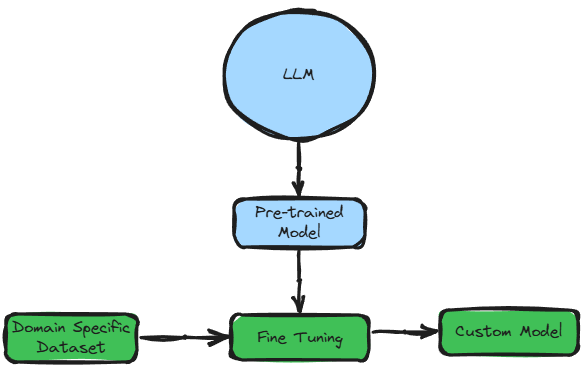
\includegraphics[width=8.5cm, height=10cm]{./imgs/fine-tuning.png}
    \caption{fine-tuning high level process}
\end{figure}

Relevant studies, like \cite{MAJIDZADEH2024103850}\cite{10298587}\cite{10298532}, had been made using fine-tuning describing different cases to apply it for software engineering capabilities like, traceability, bugfix and vulnerability detection.

\section{Methodology}

The methodology used in our study was first define a dataset with a proper format, second prepare enough data to split it in training and validation, third define how to implement a fine-tuning using a UniXcoder model, called microsoft/unixcoder-base-nine \cite{guo2022unixcoder}, and calculate precision and recall.
Since this is a very specific problem, we are creating the dataset manually, this process would be repeated until we have enough data and a good balance between precision and recall were achieved.

The dataset is choosen using public available code respecting legal copy and right rules that we can copy code for research like, Apache license 2.0, MIT and GPL.
The format used is:
\begin{itemize}
    \item content: which is real code examples.
    \item content-path: the original local path of file for tracking purposes.
    \item language: the language which the code is represented.
    \item category: design pattern, label used for classification.
    \item reference: public url from where the code was extracted.
\end{itemize}

For the training we are going to use only columns content and language as feature information and category as label information.

\subsection{Implementation}


The program will be using transformers library and microsoft\/unixcoder-base-nine\cite{guo2022unixcoder} to make fine-tuning.
Our classification uses only encoder model taking labeled code as examples to predict design patterns implemented. 
This is made by checking if the tokenized input code, which pass to the encoder layer is similar to any other samples in the trained dataset.

Also, the program structure will have some components for training, data cleanup, crawl additional data and prediction.

\begin{table}[htbp]
    \caption{Program Modules}
    \begin{center}
        \begin{tabular}{|m{2cm}|m{5.5cm}|}
            \hline
            \textbf\textbf{\textit{Module}}& \textbf{\textit{Description}} \\
            \hline 
            Samples & Initial samples labeled by human.  \\
            \hline 
            Dataset-cleaner & This module will join all data from new data recently crawled \newline 
                data and manually labeled data in a parquet file. \newline 
                Also this module remove unnecessary columns or data. \\
            \hline 
            Predictor & This module predict input from user using softmax functions. \\
            \hline 
            Trainer & Module to do fine-tuning using parquet file cleanup by Dataset-cleaner module. \\
            \hline
            Crawler & Configure repositories to crawl data and label it with pre-trained model \newline 
                for design patterns classification. \\
            \hline
        \end{tabular}
        \label{tab2}
    \end{center}
\end{table}

In the figure 1 we can see the interactions between all the modules. 
The boxes in yellow, "Human", "Public Repositories", "UniXcoder", are pieces of the system that are external to our implementation, 
but we need to generate data and have a pre-trained model to perform fine-tuning.
The boxes in blue, "Samples", "Crawler", "Dataset-cleaner", are modules that handle data. This is important since we want to guarantee data format described in Methodology to be used in our training process.

\begin{figure}[ht]
    \centering
    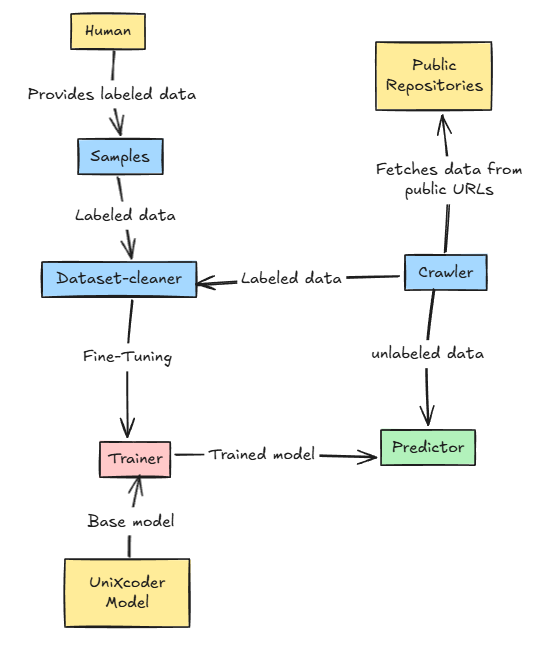
\includegraphics[width=8.6cm, height=15cm]{./imgs/modules-interaction.png}
    \caption{Experiment Architecture}
\end{figure}

\subsection{Experimental Setup}
 
To train this model we will bne using a desktop computer with AMD Ryzen 5 5600G 3.90GHz and
16GB of RAM. The initial fine-tuning takes 33 minutes using CUDA with NVIDIA RTX 3060.

\subsection{Metrics}

The trainer module was using accuracy metrics to compute metrics for each iteration. We trained our model with 21 epochs, batch size equals to 7 and learning rate of 2e-5 .
\begin{table}[htbp]
    \caption{Evaluation Metrics}
    \begin{center}
        \begin{tabular}{|m{2cm}|m{3cm}|m{2cm}|}
            \hline
            \textbf\textbf{\textit{Dataset Size}}& \textbf{\textit{Accuracy Metric}}&  \textbf{\textit{Time to train}}\\
            \hline 
            153 elements & 0.7142857142857143 & 8 minutes  \\
            \hline 
            1153 elements & 0.8947368421052632 & 00:33:14 \\
            \hline 
            3153 elements & 0.9906542056074766 & 01:19:25 \\
            \hline
        \end{tabular}
        \label{tab3}
    \end{center}
\end{table}

\section{Results}

Our final results showed that we would need to have a bigger initial dataset labeled before applying the semi-supervisioned learning process.
We can see that using our manual testing that only 224 files of 3964 files we were able to have a specific classification to determine a design pattern and other 304 of those files don't have any design pattern implemented.
This number represents 13.31 percent of the test dataset that we can properly classify. 

The reason for this to happen is because code can be very different between applications and some design patterns have a lot of similarities, which emphasize the need of having a lot of samples without the unknown label.

\section{Discussion}

Design Patterns are important piece of sofware engineering, but argualy useful sometimes. Even some studies diverging about the needs of having such kind of algorithms implemented we need to understand them, specially when maintaining legacy code.

Moving forward to make AI understanding code we need to provide useful information for AI to make code changes, create automated reparing program or even apply bugfixing, increasing the possibilities of AI generated code to keep same or better code quality.

Such information could be static analysis from the code like how UniXCoder uses Abstract Syntax Tree (AST) \cite{ZHENG2023107194} in hidden layers. But also, when creating prompts for AI to make such changes with the additional information presented in this paper. 
Automated program repairs could leverage such information not only to change code, but also to avoid risk changes without consulting human or even other data when making the changes. 



\section{Future Work}

This research have some open questions to be answered in next iterations. 
Those questions are related to, how can we calculate error propagation when applying semi-supervisioned learning, what are the models that we can classify better code for this kind of scenario and which techniquies can improve code classification.

Having a initial bigger dataset can improve a lot the f1-score of this process and also applying other techniquies, like, splitting the code in small pieces, functions, classes and attributes to help the classification and allowing it to be multi-labeled.

As we could see in this work, this problem is not straightforward and needs human validations since design patterns are implemented in very different ways across different languages and organizations.

\bibliographystyle{plain}
\bibliography{references}

\end{document}
